\documentclass[11pt,a4paper]{article}

\usepackage[T1]{fontenc}
\usepackage[utf8]{inputenc}
\usepackage[provide=*,main=french]{babel}
\usepackage{lmodern}
\usepackage{microtype}
\usepackage{geometry}
\geometry{top=2.25cm,bottom=2.35cm,left=2.35cm,right=2.35cm}
\usepackage{amsmath,amssymb,amsthm,mathtools,bm}
\usepackage{graphicx}
\usepackage{booktabs,tabularx,array,multirow}
\usepackage{enumitem}
\usepackage{xcolor}
\usepackage{caption}
\usepackage{subcaption}
\usepackage{fancyhdr}
\usepackage{hyperref}
\usepackage[nameinlink,noabbrev]{cleveref}

\definecolor{deepblue}{RGB}{21,101,192}
\definecolor{deeporange}{RGB}{216,67,21}
\definecolor{softblue}{RGB}{232,242,252}
\definecolor{softgray}{RGB}{246,247,249}
\hypersetup{
  colorlinks=true,
  linkcolor=deepblue,
  citecolor=deepblue,
  urlcolor=deeporange,
  pdftitle={Attention sphérique sans MLP : équilibres exacts et cycles},
  pdfauthor={Soumission anonyme}
}

\pagestyle{fancy}
\fancyhf{}
\fancyhead[L]{Attention sphérique sans MLP}
\fancyhead[R]{Équilibres et cycles}
\fancyfoot[C]{\thepage}
\setlength{\headheight}{14.3pt}
\setlength{\parindent}{0pt}
\setlength{\parskip}{0.52em}
\setlength{\emergencystretch}{3em}
\setcounter{tocdepth}{1}
\setlist{nosep,leftmargin=*}

\newtheorem{theorem}{Théorème}[section]
\newtheorem{proposition}[theorem]{Proposition}
\newtheorem{lemma}[theorem]{Lemme}
\newtheorem{corollary}[theorem]{Corollaire}
\theoremstyle{definition}
\newtheorem{definition}[theorem]{Définition}
\newtheorem{remark}[theorem]{Remarque}
\renewcommand{\proofname}{Preuve}

\newcommand{\sphere}{\mathbb S}
\newcommand{\R}{\mathbb R}
\newcommand{\diag}{\operatorname{diag}}
\newcommand{\Diag}{\operatorname{Diag}}
\newcommand{\rank}{\operatorname{rang}}
\newcommand{\softmax}{\operatorname{softmax}}
\newcommand{\e}{\mathrm e}
\newcommand{\T}{\mathsf T}
\newcommand{\one}{\bm 1}
\newcommand{\norm}[1]{\left\lVert #1\right\rVert}
\newcommand{\ip}[2]{\left\langle #1,#2\right\rangle}
\newcolumntype{Y}{>{\raggedright\arraybackslash}X}

\newenvironment{plainbox}
{\begin{center}\begin{minipage}{0.92\textwidth}\color{deepblue}\hrule\vspace{0.45em}\small\textbf{Lecture concrète.}\ \color{black}}
{\vspace{0.35em}\color{deepblue}\hrule\color{black}\end{minipage}\end{center}}

\newenvironment{limitbox}
{\begin{center}\begin{minipage}{0.92\textwidth}\color{deeporange}\hrule\vspace{0.45em}\small\textbf{Limite de la conclusion.}\ \color{black}}
{\vspace{0.35em}\color{deeporange}\hrule\color{black}\end{minipage}\end{center}}

\title{\textbf{Attention sphérique sans MLP :\\
équilibres exacts, multistabilité et cycle interne stable}\\[0.5em]
\large Rapport théorique et numérique reproductible}
\author{Soumission anonyme}
\date{Version du 16 août 2026}

\begin{document}
\maketitle

\begin{abstract}
Nous étudions une pile de couches réduite à son mécanisme d'attention : aucun réseau
MLP n'est présent. Chaque jeton est un point de norme un et chaque couche le déplace,
puis le renormalise. Le premier résultat est une condition nécessaire et suffisante,
valable pour tout nombre de jetons, toute dimension et toutes matrices de score et de
valeur : à l'équilibre, la moyenne transportée vue par chaque jeton doit être exactement
parallèle à ce jeton. Nous donnons sa version pour une couche finie, sa réduction par
groupes, sa linéarisation exacte et, dans le cas lié
$Q^{\T}K=V=V^{\T}$, une description complète par matrices de produits scalaires.
Cette description contient les consensus, les séparations en deux signes, les formes à
plusieurs sommets, les familles continues et les mélanges de directions propres.

Le second résultat sépare trois objets souvent confondus : un cycle de trois ou quatre
couches, un cycle continu dont le nombre de couches par tour croît comme l'inverse de
la force d'une couche, et une simple rotation rigide. Dans le cas lié symétrique, une
quantité scalaire augmente strictement et interdit tout cycle continu non constant. En
revanche, lorsque les matrices de score et de valeur sont indépendantes et que le
transport par $V$ n'est pas réciproque, l'attention seule produit un cycle interne stable
à trois jetons. Son temps de retour est $9{,}12$ dans l'unité de profondeur de l'audit ;
ses deux taux de contraction transverses sont proches de $-0{,}457$ et $-0{,}459$ ;
128 perturbations reviennent vers la même boucle. Pour sept forces de couche, dyadiques
et non dyadiques, le nombre de couches par tour suit une pente $1{,}012$ en échelle
logarithmique. Nous n'avons, à ce stade, certifié ni chaos produit par l'attention seule
ni inventaire exhaustif des cycles dans le cas non réciproque.
\end{abstract}

\begin{plainbox}
Le message en une phrase est le suivant : sans MLP, l'attention symétrique peut avoir
beaucoup de destinations stables mais elle finit par s'arrêter ; l'attention générale
peut, à elle seule, maintenir une boucle stable où les distances entre jetons changent
indéfiniment.
\end{plainbox}

\clearpage
\tableofcontents
\newpage

\section{Question étudiée et réponse courte}

Une couche Transformer usuelle contient au moins une attention, une connexion résiduelle,
une normalisation et un MLP \cite{vaswani2017attention}. Nous retirons ici complètement
le MLP. Il reste une question très précise : que peuvent faire les jetons lorsqu'on
répète uniquement l'attention et la normalisation ?

Les travaux de Geshkovski et collaborateurs ont montré que cette lecture en profondeur
comme une dynamique de particules explique la formation de groupes
\cite{geshkovski2023clusters,geshkovski2025perspective}. Altafini a classé quatre formes
d'équilibre et mis en évidence leur coexistence \cite{altafini2025multistability}.
Kuehn et Yoon ont ensuite isolé un cas plus contraint,
$Q^{\T}K=V=V^{\T}$, dans lequel les directions propres de $V$ organisent la destination
\cite{kuehnyoon2026spectral}. Notre rapport réunit ces points de vue, ferme l'équation
générale des équilibres et ajoute l'étude expérimentale des cycles sans MLP.

Les réponses sont :

\begin{enumerate}
  \item une configuration est arrêtée si et seulement si chaque jeton reçoit une somme
  qui pointe exactement dans sa direction ou dans la direction opposée ; la normalisation
  enlève alors la partie radiale et aucun angle ne change ;
  \item une forme visuellement polygonale n'est pas nécessairement un « équilibre
  polygonal » au sens d'Altafini : ce nom y désigne seulement le cas plus étroit où la
  somme reçue est nulle ;
  \item si score et valeur sont la même matrice symétrique, aucun cycle continu stable
  ne peut exister ;
  \item si l'on défait cette égalité, l'attention seule peut soutenir un cycle interne
  stable ; nous en donnons un exemple explicite et reproductible ;
  \item un cycle de période trois couches observé à grande force n'est pas la même chose
  qu'un cycle continu. Le second demande de plus en plus de couches lorsque chaque couche
  devient plus faible.
\end{enumerate}

\section{Le modèle, depuis une couche jusqu'au temps continu}
\label{sec:model}

\subsection{Ce que représentent les symboles}

Il y a $n$ jetons. Le jeton $i$ est un vecteur $x_i\in\R^d$ de norme un. Il vit donc sur
la sphère $\sphere^{d-1}$. Deux matrices suffisent :

\begin{itemize}
  \item $S=Q^{\T}K$ décide qui regarde qui ;
  \item $V$ décide quel vecteur est effectivement transporté.
\end{itemize}

Le nombre $\beta\geq0$ règle la netteté du choix. Pour $\beta=0$, tous les jetons sont
pondérés de la même façon. Lorsque $\beta$ augmente, les différences de scores comptent
davantage. Pour une configuration $X=(x_1,\ldots,x_n)$, posons

\begin{align}
 s_{ij}(X)&=x_i^{\T}Sx_j,\\
 a_{ij}(X)&=\frac{\exp(\beta s_{ij}(X))}
 {\sum_{k=1}^n\exp(\beta s_{ik}(X))},\\
 y_i(X)&=\sum_{j=1}^n a_{ij}(X)Vx_j. \label{eq:attention-output}
\end{align}

$a_{ij}$ est le poids donné par $i$ à $j$, et $y_i$ est la somme reçue par $i$ après le
transport par $V$.

\subsection{Une couche finie}

Sans MLP, la couche résiduelle normalisée est exactement
\begin{equation}
 x_i^+=\frac{x_i+h y_i(X)}{\norm{x_i+h y_i(X)}} ,
 \qquad i=1,\ldots,n,                                      \label{eq:finite-map}
\end{equation}
où $h>0$ est la force d'une couche. Cette normalisation sur la sphère est une version
idéalisée de RMSNorm \cite{zhang2019rmsnorm}.

\subsection{Beaucoup de couches faibles}

Écrivons
\[
 P_x=I-xx^{\T}.
\]
$P_xz$ garde seulement la partie de $z$ qui change la direction de $x$ ; la partie
parallèle à $x$ changerait seulement sa longueur et sera supprimée par la normalisation.
Le développement de \eqref{eq:finite-map} donne
\[
 x_i^+=x_i+hP_{x_i}y_i(X)+O(h^2).
\]
Si le nombre de couches croît pendant que $h$ décroît, la limite est
\begin{equation}
 \boxed{\quad \dot x_i=P_{x_i}y_i(X)
 =y_i(X)-\bigl(x_i^{\T}y_i(X)\bigr)x_i.\quad}              \label{eq:ode}
\end{equation}
La norme reste égale à un car $x_i^{\T}\dot x_i=0$.

Sur le cercle, on écrit $x_i=(\cos\theta_i,\sin\theta_i)$ et
$t_i=(-\sin\theta_i,\cos\theta_i)$. L'équation devient un seul nombre par jeton :
\begin{equation}
 \dot\theta_i=\sum_{j=1}^n a_{ij}(\theta)\,t_i^{\T}Vx_j.  \label{eq:circle}
\end{equation}
Toutes les expériences de cycle de ce rapport utilisent cette équation à trois jetons.

\section{La condition finale de tous les équilibres}
\label{sec:equilibria}

\begin{theorem}[Condition nécessaire et suffisante, matrices générales]
\label{thm:general-equilibrium}
Une configuration $X\in(\sphere^{d-1})^n$ est un équilibre de
\eqref{eq:ode} si et seulement si, pour chaque jeton $i$,
\begin{equation}
 \boxed{\quad y_i(X)=\lambda_i x_i,
 \qquad \lambda_i=x_i^{\T}y_i(X).\quad}                   \label{eq:parallel-condition}
\end{equation}
De façon équivalente, sans dénominateur softmax,
\begin{equation}
 \boxed{\quad
 \sum_{j=1}^n \e^{\beta x_i^{\T}Sx_j}
 \left[Vx_j-\bigl(x_i^{\T}Vx_j\bigr)x_i\right]=0,
 \qquad i=1,\ldots,n.\quad}                               \label{eq:final-equilibrium}
\end{equation}
\end{theorem}

\begin{proof}
Le champ est $P_{x_i}y_i$. Il est nul exactement lorsque $y_i$ appartient à la droite
portée par $x_i$. Le coefficient de cette colinéarité est son produit scalaire avec
$x_i$. Enfin, le dénominateur du softmax est strictement positif ; le multiplier ou le
supprimer ne change donc pas l'égalité à zéro.
\end{proof}

\begin{plainbox}
Il n'est pas nécessaire que la somme reçue soit nulle. Elle peut être grande. Il suffit
qu'elle pousse exactement vers le centre ou vers l'extérieur le long du rayon du jeton.
La renormalisation efface cette poussée radiale. C'est la raison simple pour laquelle des
formes à plusieurs sommets peuvent être stables.
\end{plainbox}

\subsection{La condition exacte pour une couche finie}

\begin{proposition}[Point fixe de la couche]
Supposons $x_i+h y_i\neq0$. La couche \eqref{eq:finite-map} laisse $x_i$ inchangé si et
seulement si
\begin{equation}
 P_{x_i}y_i=0
 \quad\text{et}\quad
 1+h\lambda_i>0,
 \qquad \lambda_i=x_i^{\T}y_i.                             \label{eq:finite-fixed}
\end{equation}
\end{proposition}

La première condition est la même que pour le temps continu. La seconde est propre à
une couche finie : si $1+h\lambda_i<0$, la normalisation retourne le point antipodal
$-x_i$ ; si $1+h\lambda_i=0$, elle tente de normaliser le vecteur nul.

\subsection{Réduction exacte lorsque plusieurs jetons coïncident}

Supposons que la configuration contienne seulement $q$ positions distinctes
$w_1,\ldots,w_q$, répétées respectivement $r_1,\ldots,r_q$ fois. Alors
\eqref{eq:final-equilibrium} devient le système fini
\begin{equation}
 \boxed{\quad
 \sum_{b=1}^q r_b\e^{\beta w_a^{\T}Sw_b}
 \left[Vw_b-\bigl(w_a^{\T}Vw_b\bigr)w_a\right]=0,
 \quad a=1,\ldots,q.\quad}                                \label{eq:cluster-reduction}
\end{equation}
Ce n'est pas une approximation. On a seulement regroupé des termes identiques. Pour une
instance fixée, \eqref{eq:cluster-reduction} donne une procédure exhaustive : énumérer
les partitions $r_1+\cdots+r_q=n$, résoudre les équations, puis retirer les copies obtenues
par permutation.

\subsection{Pourquoi le mot « polygone » a créé une confusion}
\label{sec:terminology}

Altafini \cite{altafini2025multistability} emploie quatre noms. La distinction utile est
résumée dans le \cref{tab:altafini-classes}.

\begin{table}[ht]
\centering
\caption{Les quatre noms d'Altafini, exprimés avec la somme $y_i$ de
\eqref{eq:attention-output}. Les deux dernières lignes couvrent toutes les formes non
colinéaires.}
\label{tab:altafini-classes}
\begin{tabularx}{\textwidth}{@{}lXl@{}}
\toprule
Nom & Configuration & Condition reçue \\
\midrule
Consensus & tous les $x_i$ sont égaux à une direction propre de $V$ & $y_i\parallel x_i$ \\
Consensus bipolaire & chaque $x_i$ vaut $u$ ou $-u$, avec $u$ propre & $y_i\parallel x_i$ \\
Polygonal & plusieurs directions, et aucune sortie & $y_i=0$ pour tout $i$ \\
Clustering & tout autre équilibre, avec ou sans jetons coïncidents & $y_i=\lambda_i x_i$, au moins un $\lambda_i\neq0$ \\
\bottomrule
\end{tabularx}
\end{table}

Ainsi, « les points dessinent un triangle » est une description visuelle. « Polygonal »
au sens du théorème d'Altafini est une condition algébrique beaucoup plus étroite. Un
triangle dont les trois sorties sont non nulles et radiales appartient à sa quatrième
classe. L'instabilité des sorties nulles ne dit rien contre la stabilité de ce triangle.

\section{Cas lié symétrique : une description complète}
\label{sec:symmetric}

Nous imposons maintenant
\begin{equation}
 S=V=V^{\T}.                                                \label{eq:tied-symmetry}
\end{equation}
C'est exactement l'hypothèse de Kuehn--Yoon
\cite{kuehnyoon2026spectral}. Elle est plus forte que celle d'Altafini : Altafini suppose
$V$ symétrique avec une valeur propre positive dominante simple, mais ne demande pas que
$Q^{\T}K$ soit symétrique ni égal à $V$.

Écrivons les jetons comme les lignes d'une matrice $X\in\R^{n\times d}$ et posons
\[
 H=XVX^{\T},\qquad R=\exp_\circ(\beta H),
\]
où l'exponentielle est appliquée entrée par entrée. Définissons
\[
 M=\Diag\bigl(\diag(RH)\bigr).
\]

\begin{theorem}[Équation vectorielle complète]
\label{thm:vector-complete}
Sous \eqref{eq:tied-symmetry},
\begin{equation}
 \boxed{\quad X\text{ est un équilibre}
 \iff RXV=MX,qquad \diag(XX^{\T})=\one.\quad}              \label{eq:matrix-equilibrium}
\end{equation}
\end{theorem}

Cette formule est déjà nécessaire et suffisante. La suivante retire les rotations qui ne
changent pas le problème.

\begin{theorem}[Description spectrale par produits scalaires]
\label{thm:spectral-gram}
Soient $\lambda_1^\star,\ldots,\lambda_s^\star$ les valeurs propres distinctes de $V$,
de multiplicités $m_1,\ldots,m_s$. Écrivons la partie de $X$ dans chaque espace propre
sous la forme $C_\alpha\in\R^{n\times m_\alpha}$ et posons
$G_\alpha=C_\alpha C_\alpha^{\T}$. Modulo les rotations internes aux espaces propres,
les équilibres sont exactement les familles $(G_\alpha)$ satisfaisant
\begin{equation}
\boxed{
\begin{aligned}
 &G_\alpha\succeq0,qquad \rank G_\alpha\le m_\alpha,\\
 &\sum_{\alpha=1}^s\diag G_\alpha=\one,\\
 &H=\sum_{\alpha=1}^s\lambda_\alpha^\star G_\alpha,
 \qquad R=\exp_\circ(\beta H),\\
 &M=\Diag\bigl(\diag(RH)\bigr),\\
 &(\lambda_\alpha^\star R-M)G_\alpha=0,
 \qquad \alpha=1,\ldots,s.
\end{aligned}}                                             \label{eq:spectral-gram}
\end{equation}
\end{theorem}

La preuve, donnée en \cref{app:proofs}, consiste seulement à projeter
\eqref{eq:matrix-equilibrium} sur chaque espace propre puis à factoriser les matrices
$G_\alpha$. Le système \eqref{eq:spectral-gram} est une caractérisation complète, pas
une liste de formes choisies à l'avance.

\subsection{Toutes les familles universelles contenues dans la condition}

Le \cref{tab:families} donne les branches qui existent sans résoudre numériquement un
cas particulier.

\begin{table}[ht]
\centering
\caption{Familles exactes sans MLP sous l'hypothèse liée symétrique.}
\label{tab:families}
\begin{tabularx}{\textwidth}{@{}lX@{}}
\toprule
Situation & Tous les équilibres ou familles immédiatement garantis \\
\midrule
$V=0$ & toute configuration de $(\sphere^{d-1})^n$ \\
Un jeton & toutes les sphères unités contenues dans les espaces propres de $V$ \\
Consensus & $x_1=\cdots=x_n=u$ pour toute direction propre unitaire $u$ \\
Une droite propre & tout motif $x_i\in\{u,-u\}$ \\
Noyau de $V$ & toute configuration contenue dans $\ker V$ ; des ajouts mixtes sont possibles si la sortie active s'annule \\
Un espace propre multiple & simplexes réguliers, polygones réguliers, hypercubes et autres orbites symétriques, avec multiplicités compatibles \\
Plusieurs espaces propres & branches mixtes, symétriques ou asymétriques, résolues par \eqref{eq:spectral-gram} ou \eqref{eq:cluster-reduction} \\
\bottomrule
\end{tabularx}
\end{table}

Il n'existe donc pas de liste finie valable pour tout $n,d,V$ : si $V=0$, chaque point
est un équilibre ; si une valeur propre est multiple, des familles continues apparaissent.
La bonne notion de « tous les équilibres » est la condition constructive
\eqref{eq:spectral-gram}.

\subsection{Classification entièrement explicite lorsque \texorpdfstring{$\beta=0$}{bêta = 0}}

À $\beta=0$, les poids valent tous $1/n$. Posons
\[
 z=V\sum_{j=1}^n x_j.
\]

\begin{theorem}[Tous les équilibres à attention uniforme]
\label{thm:beta-zero}
Pour une matrice $V$ quelconque, une configuration est un équilibre si et seulement si
l'une des deux situations suivantes se produit :
\begin{enumerate}
  \item $z=0$ ; toute configuration telle que $V\sum_jx_j=0$ convient ;
  \item $z\neq0$ ; tous les jetons valent $u$ ou $-u$, leur somme signée est non nulle,
  et $u$ est un vecteur propre réel de $V$ associé à une valeur propre non nulle.
\end{enumerate}
\end{theorem}

Cette classification montre à la fois la richesse et la fragilité du cas uniforme. Avec
une matrice symétrique, il s'agit d'une dynamique d'énergie. Avec une matrice non
symétrique, une rotation peut subsister même si les poids ne changent jamais.

\subsection{Une famille mixte exacte à trois groupes}

Soient $Vu=au$, $Vv=bv$, avec $u\perp v$. Prenons $m$ copies de $u$, $k$ copies de
$qu+\sqrt{1-q^2}v$ et $k$ copies de $qu-\sqrt{1-q^2}v$. Cette forme est un équilibre
exactement lorsque
\begin{equation}
\boxed{
q\left[(a-b)\e^{\beta[b+(a-b)q^2]}
 +(a+b)\e^{\beta[-b+(a+b)q^2]}\right]
 +a\frac{m}{k}\e^{\beta aq}=0.}                           \label{eq:mixed-family}
\end{equation}
Cette seule équation produit des branches qui utilisent simultanément deux directions
propres. Elle explique pourquoi « choisir une seule valeur propre » ne suffit pas à
décrire toutes les destinations.

\section{Quand un équilibre attire-t-il les trajectoires ?}
\label{sec:stability}

La condition \eqref{eq:final-equilibrium} dit où la dynamique peut s'arrêter. La
stabilité dit ce qui se passe après une petite erreur de position.

Soit $\delta x_i$ une petite variation perpendiculaire à $x_i$. Définissons
\begin{align}
 \delta s_{ij}
 &=\delta x_i^{\T}Sx_j+x_i^{\T}S\delta x_j,\\
 \delta a_{ij}
 &=\beta a_{ij}\left(\delta s_{ij}-\sum_k a_{ik}\delta s_{ik}\right),\\
 \delta y_i
 &=\sum_j a_{ij}V\delta x_j+\sum_j\delta a_{ij}Vx_j.       \label{eq:variations}
\end{align}
À un équilibre $y_i=\lambda_i x_i$, la variation tangentielle du champ est
\begin{equation}
 \boxed{\quad \delta\dot x_i=P_{x_i}\delta y_i-\lambda_i\delta x_i.\quad}
                                                                    \label{eq:tangent-jacobian}
\end{equation}
Ces lignes donnent la matrice de stabilité exacte pour toutes matrices $S,V$. L'équilibre
attire localement si toutes ses valeurs propres tangentielles ont une partie réelle
strictement négative. Une valeur nulle peut simplement correspondre à une famille
continue obtenue par rotation ; elle doit alors être retirée avant de conclure.

\subsection{Directions propres pures dans le cas lié symétrique}

Pour un consensus $x_i=u$ sur une valeur propre $\lambda_p$, la condition locale est
particulièrement simple :
\begin{equation}
 \lambda_p>0,qquad \lambda_k<\lambda_p\quad(k\neq p).      \label{eq:consensus-stable}
\end{equation}
Le consensus stable utilise donc la plus grande valeur propre positive simple.

Pour un partage équilibré entre $u$ et $-u$, les seuils sont :
\begin{align}
 &\lambda_p>0:
 &&\lambda_k<\lambda_p\tanh(\beta\lambda_p)
 &&\text{pour tout }k\neq p,                              \label{eq:positive-bipolar}\\
 &\lambda_p<0:
 &&\lambda_p<\lambda_k<\lambda_p\tanh(\beta\lambda_p)
 &&\text{pour tout }k\neq p.                              \label{eq:negative-bipolar}
\end{align}
Le second cas sélectionne nécessairement la valeur propre la plus négative. Les formules
pour un partage déséquilibré sont données en \cref{app:imbalanced}.

\subsection{Un triangle stable qui n'est pas « polygonal » au sens d'Altafini}

Pour $V=S=\Diag(2,-3)$, $\beta=1{,}5$ et trois jetons, la recherche de racines trouve la
configuration d'angles, arrondie ici,
\[
 (0,\;1{,}546889,\;4{,}736296).
\]
Son taux linéaire le moins contractant vaut $-0{,}9144$ et le résidu calculé avant arrondi
est $1{,}3\times10^{-15}$. Surtout, les longueurs des trois sorties non normalisées valent
environ $40{,}27$, $269{,}79$ et $269{,}79$ : elles ne sont pas nulles. Elles pointent
radialement. Ce triangle est donc stable et appartient à la classe « clustering »
d'Altafini, pas à sa classe « polygonal ».

La recherche multi-départ de petits systèmes donne le \cref{fig:small-catalogue}.
Deux graines indépendantes retrouvent exactement les mêmes ensembles après retrait des
permutations et du changement de signe global.

\begin{figure}[ht]
\centering
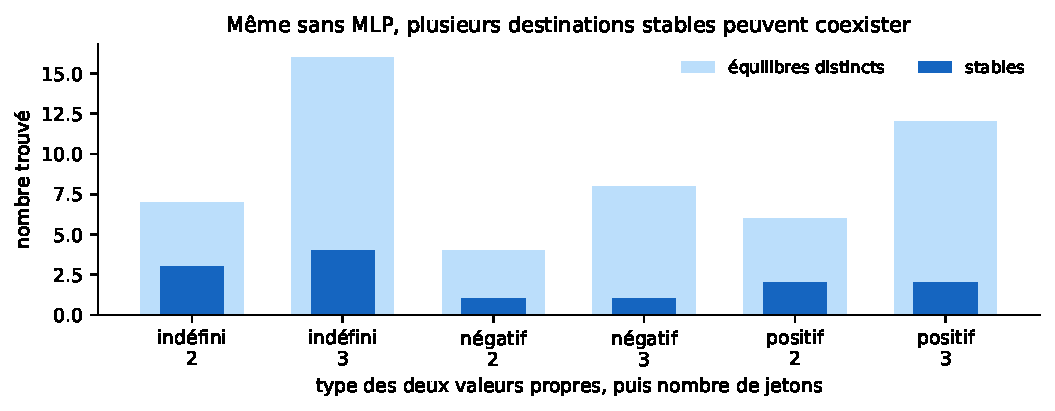
\includegraphics[width=0.92\textwidth]{figures/small_equilibrium_catalogue.pdf}
\caption{Catalogue sans MLP pour $V=S$ symétrique en dimension deux. Les spectres sont
$(2,-3)$ avec $\beta=1{,}5$, $(-0{,}4,-4)$ avec $\beta=0{,}03$, et $(3,2)$ avec
$\beta=1{,}5$. Les nombres au second niveau des étiquettes sont les nombres de jetons.
La recherche numérique découvre les branches ; la complétude théorique vient de
\eqref{eq:spectral-gram}, pas du nombre de départs.}
\label{fig:small-catalogue}
\end{figure}

\section{Cycles : trois objets qu'il faut séparer}
\label{sec:cycles}

\subsection{Cycle court d'une couche finie}

Un cycle de période $p$ de la couche est une suite de $p$ configurations distinctes qui
revient exactement au départ après $p$ applications de \eqref{eq:finite-map}. Cet objet
dépend de la force $h$.

\begin{lemma}[Un nombre fixe de couches ne survit pas tel quel]
\label{lem:fixed-period}
Si la couche satisfait $F_h(X)=X+h f(X)+O(h^2)$ et si $p$ reste fixe lorsque $h\to0$,
alors toute limite d'un cycle de période $p$ vérifie $f(X)=0$.
\end{lemma}

En effet, $F_h^p(X)=X+phf(X)+O(h^2)$. Un cycle de trois couches peut donc se contracter
vers un équilibre quand on rend les couches faibles. Il ne prouve pas l'existence d'une
boucle en temps continu.

\subsection{Cycle continu}

Un cycle continu est une boucle parcourue en un temps $T>0$. Une couche de force $h$
n'en parcourt qu'une fraction. Le nombre de couches par tour doit donc croître comme
$T/h$. C'est la signature mesurée dans le \cref{fig:cycle-stability-depth}.

\subsection{Rotation rigide et cycle interne}

Si tous les produits scalaires $x_i^{\T}x_j$ restent constants pendant que l'ensemble
tourne, la forme n'évolue pas : c'est une rotation rigide. Dans un cycle interne, au moins
une distance entre jetons change puis revient. Cette seconde situation est plus forte.

Un exemple analytique montre déjà que l'attention sans MLP peut tourner. Prenons un seul
jeton sur le cercle, $S=0$ et
\[
 V=\omega\begin{pmatrix}0&-1\\1&0\end{pmatrix}.
\]
Alors $\dot x=Vx$ et le jeton tourne avec période $2\pi/|\omega|$. Cette rotation est
neutre : elle ne prouve pas qu'une boucle attire les perturbations. L'expérience de la
\cref{sec:cycle-experiment} établit précisément ce point plus difficile.

\section{Pourquoi la symétrie interdit les cycles continus}
\label{sec:no-cycle}

Sous $S=V=V^{\T}$ et pour $\beta>0$, définissons
\begin{equation}
 E_\beta(X)=\frac{1}{2\beta}\sum_{i,j=1}^n
 \exp\!\left(\beta x_i^{\T}Vx_j\right).                   \label{eq:energy}
\end{equation}
Si $Z_i=\sum_j\exp(\beta x_i^{\T}Vx_j)$, un calcul direct donne
\begin{equation}
 \frac{dE_\beta}{dt}=\sum_{i=1}^n Z_i\norm{\dot x_i}^2\geq0.  \label{eq:energy-growth}
\end{equation}
La quantité augmente strictement dès qu'un jeton bouge. Une trajectoire fermée devrait
revenir à sa valeur initiale de $E_\beta$, ce qui est impossible sauf si elle est déjà
arrêtée. Ce mécanisme est la structure de gradient pondéré utilisée par
Kuehn--Yoon \cite{kuehnyoon2026spectral}.

À $\beta=0$, la même conclusion vaut avec
\[
 \Phi(X)=\frac{1}{2n}\left(\sum_i x_i\right)^{\T}
 V\left(\sum_jx_j\right).
\]

\begin{plainbox}
La symétrie importante n'est pas seulement « $V$ est symétrique ». Il faut, pour cette
preuve, que la matrice qui calcule les scores soit la même que celle qui transporte les
valeurs : $S=V=V^{\T}$. Si $S$ et $V$ sont indépendantes, l'argument disparaît.
\end{plainbox}

Sur le cercle à $\beta=0$, l'écart à la réciprocité se voit exactement dans
\begin{equation}
 \frac{\partial\dot\theta_i}{\partial\theta_j}
 -\frac{\partial\dot\theta_j}{\partial\theta_i}
 =\frac1n t_i^{\T}(V-V^{\T})t_j.                          \label{eq:curl}
\end{equation}
La partie antisymétrique de $V$ fournit donc une circulation. À $\beta>0$, la
normalisation ligne par ligne des poids ajoute des termes supplémentaires. Même lorsque
les dérivées croisées ordinaires ne coïncident pas, le cas $S=V=V^{\T}$ reste sans cycle
grâce à la métrique pondérée de \eqref{eq:energy-growth}. Ce détail évite de confondre
« gradient euclidien » et « quantité monotone ».

\section{Expérience centrale : un cycle stable produit par l'attention seule}
\label{sec:cycle-experiment}

\subsection{Paramètres explicites}

Le modèle utilise trois jetons sur le cercle, aucun MLP, et
\begin{equation}
S=\begin{pmatrix}
1{,}112495&1{,}768642\\
-2{,}540753&3{,}294286
\end{pmatrix},\qquad
V=\begin{pmatrix}
-1{,}809502&1{,}419182\\
-1{,}827949&-3{,}611608
\end{pmatrix},                                             \label{eq:cycle-matrices}
\end{equation}
avec $\beta=1{,}110063$. L'audit mesure la profondeur avec une échelle
$\rho=0{,}551488$ : son équation est $\dot\theta_i=\rho\sum_j a_{ij}t_i^{\T}Vx_j$.
Absorber $\rho$ dans le temps ramène exactement à \eqref{eq:circle}.

Ce modèle a été isolé par ablation d'un candidat provenant d'un écran plus large avec
MLP. Après suppression de tous les paramètres MLP, le cycle reste présent. Le MLP seul,
avec l'attention supprimée, converge au contraire vers un point fixe. Cette sélection du
modèle doit être gardée en tête : elle démontre l'existence d'un cycle d'attention, pas sa
fréquence dans une loi aléatoire de matrices.

\subsection{La forme change pendant le tour}

La réintégration indépendante par Runge--Kutta d'ordre quatre, avec pas $0{,}005$, donne
un temps de retour $T=9{,}12$ en profondeur normalisée, soit $5{,}030$ dans le temps de
\eqref{eq:circle} après absorption de $\rho$. Le résidu de retour au quantile 90\% est
$1{,}56\times10^{-3}$ radian.

\begin{figure}[ht]
\centering
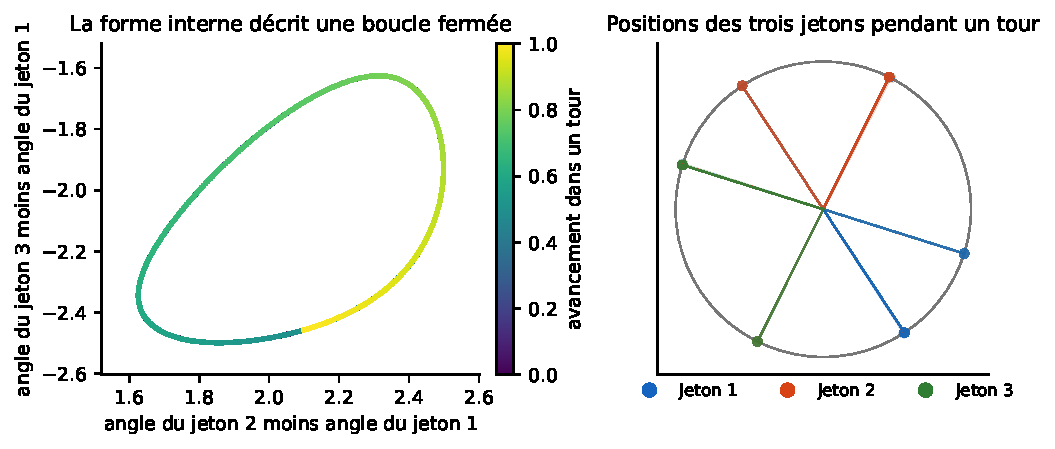
\includegraphics[width=\textwidth]{figures/attention_only_cycle_geometry.pdf}
\caption{Cycle interne de l'attention seule. À gauche, les deux angles relatifs décrivent
une boucle fermée ; une rotation rigide serait un point. À droite, sept phases d'un tour
montrent les trois jetons sur le cercle. Les angles sont toujours pris modulo $2\pi$.}
\label{fig:cycle-geometry}
\end{figure}

Les trois produits scalaires entre paires varient chacun de $-0{,}8002$ à $-0{,}0551$.
La forme change donc fortement. Les poids envoyés par le jeton 1 vers les jetons 1, 2 et
3 parcourent respectivement les intervalles
\[
[0{,}298,0{,}982],\qquad[0{,}015,0{,}701],\qquad
[0{,}00018,0{,}0341].
\]

\begin{figure}[ht]
\centering
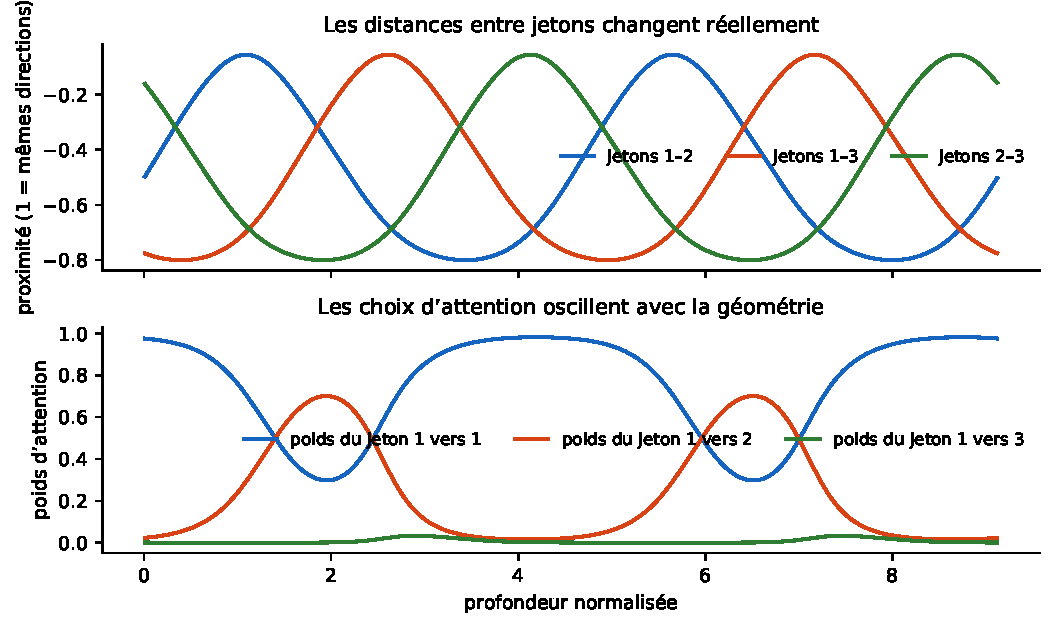
\includegraphics[width=\textwidth]{figures/attention_only_cycle_observables.pdf}
\caption{Un tour du cycle. En haut, les produits scalaires entre jetons oscillent ; en
bas, les poids de la première ligne d'attention oscillent eux aussi. La deuxième période
visible dans les distances provient d'une permutation de rôle entre jetons au cours du
retour complet des angles étiquetés.}
\label{fig:cycle-observables}
\end{figure}

\subsection{Pourquoi nous l'appelons stable}

Sur une boucle autonome, une variation qui avance simplement la phase n'est ni contractée
ni amplifiée : son taux théorique est zéro. Le spectre mesuré sur 2000 unités est
\begin{equation}
 (-0{,}00273,\;-0{,}45676,\;-0{,}45937).                   \label{eq:cycle-spectrum}
\end{equation}
Le premier nombre est l'approximation finie du zéro de phase. Les deux autres sont
nettement négatifs : les écarts perpendiculaires à la boucle se contractent.

Nous avons également ajouté 128 perturbations gaussiennes d'écart-type $0{,}08$ autour
d'un point du cycle. La médiane de la distance à toute la boucle passe de $0{,}0525$ à
$0{,}00194$ ; son quantile 90\% passe de $0{,}0938$ à $0{,}00320$. Le plateau final est
du même ordre que l'espacement utilisé pour stocker la boucle de référence.

\subsection{Le tour demande bien un nombre de couches proportionnel à \texorpdfstring{$1/h$}{1/h}}

Nous avons rejoué la couche exacte \eqref{eq:finite-map} pour sept ratios, dont trois
non dyadiques. Le \cref{tab:period-scaling} donne le meilleur retour complet.

\begin{table}[ht]
\centering
\caption{Retour du cycle de l'attention seule lorsque chaque couche est affaiblie. Le
temps d'un tour est le nombre de couches multiplié par le ratio.}
\label{tab:period-scaling}
\begin{tabular}{@{}rrrr@{}}
\toprule
Ratio & Couches par tour & Temps du tour & Erreur angulaire maximale \\
\midrule
$1/16$   & 138  & 8,625 & $2{,}38\times10^{-2}$ \\
$1/31$   & 275  & 8,871 & $9{,}46\times10^{-3}$ \\
$1/64$   & 576  & 9,000 & $5{,}38\times10^{-3}$ \\
$1/127$  & 1151 & 9,063 & $5{,}43\times10^{-5}$ \\
$1/256$  & 2328 & 9,094 & $1{,}13\times10^{-3}$ \\
$1/509$  & 4635 & 9,106 & $7{,}42\times10^{-4}$ \\
$1/1024$ & 9333 & 9,114 & $1{,}09\times10^{-5}$ \\
\bottomrule
\end{tabular}
\end{table}

La pente de $\log(\text{couches par tour})$ en fonction de
$\log(1/\text{ratio})$ vaut $1{,}012$. Le temps du tour tend vers celui de l'équation
continue, tandis que le nombre de couches diverge.

\begin{figure}[ht]
\centering
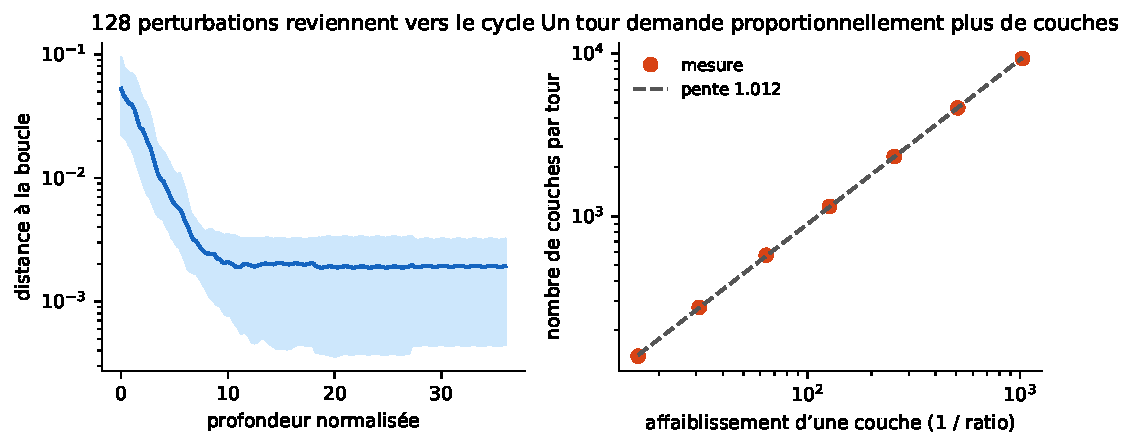
\includegraphics[width=\textwidth]{figures/attention_only_cycle_stability_depth.pdf}
\caption{À gauche, contraction de 128 perturbations vers la boucle. La ligne est la
médiane et la zone contient 80\% des essais. À droite, nombre de couches par tour ; la
pente proche de un est la signature d'un cycle continu, et non d'un artefact à trois ou
quatre couches.}
\label{fig:cycle-stability-depth}
\end{figure}

\subsection{Ce que les autres ablations ont donné}

Le \cref{tab:ablations} empêche une conclusion trop large. Les trois candidats chaotiques
les plus étudiés ne restent pas chaotiques lorsque le MLP est supprimé ; ils convergent à
un équilibre dans l'ablation attention seule.

\begin{table}[ht]
\centering
\caption{Résultat des ablations attention seule sur les représentants étudiés en détail.}
\label{tab:ablations}
\begin{tabularx}{\textwidth}{@{}lXl@{}}
\toprule
Origine du représentant & Structure de l'attention & Résultat sans MLP \\
\midrule
Cycle à trois jetons, indice 1323 & $S$ général, $V$ général, $\beta>0$ & cycle interne stable \\
Chaos fort à trois jetons, indice 2612 & $S$ symétrique, $V$ général, $\beta>0$ & consensus fixe \\
Chaos faible à trois jetons, indice 1051 & $S=V=V^{\T}$, $\beta>0$ & consensus fixe \\
Intermittence à quatre jetons, indice 3118 & $S$ symétrique, $V$ général, $\beta=0$ & équilibre fixe \\
\bottomrule
\end{tabularx}
\end{table}

\begin{limitbox}
Nous avons certifié l'existence d'un cycle interne stable produit par l'attention seule.
Nous n'avons pas encore effectué un recensement aléatoire exhaustif dédié uniquement à
l'attention générale. Nous ne concluons donc ni que ce cycle est unique, ni qu'il est
fréquent. Aucune des ablations ciblées ne fournit à ce jour un attracteur chaotique
d'attention seule.
\end{limitbox}

\section{Comparaison exacte avec Altafini et Kuehn--Yoon}
\label{sec:comparison}

\subsection{Ce qu'Altafini suppose réellement}

Le modèle d'Altafini contient bien les matrices $Q$ et $K$. Son analyse principale
suppose :
\begin{equation}
 V=V^{\T},\qquad \lambda_1>0\text{ simple et strictement dominante}.  \label{eq:altafini-assumption}
\end{equation}
Elle ne suppose pas $Q^{\T}K$ symétrique. Sous ces conditions, Altafini prouve que les
équilibres à sortie nulle qu'il appelle polygonaux sont instables. Il montre aussi que des
consensus bipolaires et des équilibres de regroupement peuvent être stables et coexister.

\subsection{Pourquoi nos résultats ne contredisent pas ce théorème}

Il y a trois raisons indépendantes :

\begin{enumerate}
  \item le triangle stable de la \cref{sec:stability} a des sorties non nulles. Il est dans
  la classe « clustering » d'Altafini, que son théorème n'annonce pas instable ;
  \item les branches négatives définies de Kuehn--Yoon n'ont aucune valeur propre
  positive et sortent donc de \eqref{eq:altafini-assumption} ;
  \item le cycle de \eqref{eq:cycle-matrices} utilise un $V$ non symétrique et n'est pas
  un équilibre. Il sort à la fois de l'hypothèse sur $V$ et de la question « stabilité d'un
  équilibre polygonal ».
\end{enumerate}

\subsection{Ce que l'hypothèse de Kuehn--Yoon ajoute}

Kuehn--Yoon imposent la relation plus forte
\[
 Q^{\T}K=V=V^{\T}.
\]
Elle fournit la quantité monotone \eqref{eq:energy}. Leur article établit des résultats
globaux de sélection dans un cône lorsque la valeur propre positive dominante dépasse en
module les autres, et pour deux jetons lorsque $V$ est négative définie
\cite{kuehnyoon2026spectral}. Notre caractérisation \eqref{eq:spectral-gram} complète la
question différente « quels sont tous les points d'arrêt possibles ? », y compris les
branches mixtes et les multiplicités, sans prétendre que chacun est atteint depuis une
initialisation générique.

\begin{table}[ht]
\centering
\caption{Portée des trois analyses.}
\label{tab:scope}
\begin{tabularx}{\textwidth}{@{}lYYY@{}}
\toprule
 & Altafini & Kuehn--Yoon & Présent rapport \\
\midrule
MLP & absent & absent & absent \\
Score $S=Q^{\T}K$ & général & égal à $V$ & général, puis cas égal à $V$ \\
Valeur $V$ & symétrique, sommet positif simple & symétrique, spectres ciblés & générale ; classification complète si liée symétrique \\
Équilibres & quatre classes, seuils sur branches pures & sélection spectrale et stabilité pure & condition nécessaire et suffisante, réduction par groupes, système spectral--Gram \\
Cycles & cycle possible signalé si $V$ perd la symétrie & interdits par l'énergie & cycle interne stable explicite sans MLP \\
\bottomrule
\end{tabularx}
\end{table}

\section{Ce qui est nouveau, dit simplement}
\label{sec:new}

\begin{enumerate}
  \item \textbf{Une seule équation couvre toutes les destinations.} Les consensus, les
  deux groupes opposés, les triangles, les formes asymétriques et les familles continues
  sont tous les cas de \eqref{eq:final-equilibrium}. La somme n'a pas besoin de s'annuler ;
  elle doit seulement être radiale.

  \item \textbf{Le mot polygone ne décide pas de la stabilité.} Un dessin à plusieurs
  sommets peut être stable lorsque les sorties sont non nulles. L'affirmation
  « polygonal instable » d'Altafini concerne uniquement les sorties exactement nulles.

  \item \textbf{Sans MLP ne veut pas dire sans mouvement durable.} L'égalité
  $Q^{\T}K=V=V^{\T}$ force l'arrêt, mais une tête générale peut entretenir seule un cycle
  où les distances et les poids d'attention oscillent.

  \item \textbf{Nous savons distinguer une boucle réelle d'un tour de passe-passe de
  discrétisation.} Dans notre cycle, affaiblir une couche multiplie le nombre de couches
  nécessaires par le facteur inverse, tout en gardant le temps d'un tour proche de
  $9{,}12$.

  \item \textbf{Le résultat est une existence, pas encore une statistique universelle.}
  Un cycle stable est certifié ; aucun chaos sans MLP ne l'est. La fréquence de ces cycles
  pour des matrices aléatoires reste une expérience fondamentale à faire.
\end{enumerate}

\section{Conclusion}

Le système sans MLP est déjà assez riche pour avoir plusieurs destinations stables et,
si la réciprocité est brisée, une oscillation interne stable. La frontière théorique est
simple. Lorsque la même matrice symétrique calcule les scores et transporte les valeurs,
une quantité augmente à chaque mouvement : les jetons doivent finir par s'arrêter. Quand
les deux rôles sont séparés, cette barrière disparaît ; les sommes reçues peuvent se
relancer mutuellement autour d'une boucle.

La condition finale à retenir est \eqref{eq:final-equilibrium}. Elle est exacte dans toute
dimension. Elle dit ce qu'il faut résoudre pour énumérer les équilibres, ce qu'il faut
différencier pour tester leur stabilité, et pourquoi une forme à plusieurs sommets peut
être stable sans contredire Altafini. Le cycle explicite montre ensuite que les équilibres
ne sont pas toute l'histoire dès que $S$ et $V$ ne sont plus liés par la symétrie forte de
Kuehn--Yoon.

\appendix

\section{Preuves complémentaires}
\label{app:proofs}

\subsection{Preuve du théorème spectral--Gram}

Dans une base propre de $V$, écrivons $X=C_1\oplus\cdots\oplus C_s$. L'équation
$RXV=MX$ projetée sur l'espace de valeur propre $\lambda_\alpha^\star$ devient
\[
 (\lambda_\alpha^\star R-M)C_\alpha=0.
\]
En multipliant à droite par $C_\alpha^{\T}$, on obtient
$(\lambda_\alpha^\star R-M)G_\alpha=0$. Les identités sur $H$ et les diagonales suivent
de la décomposition orthogonale.

Réciproquement, factorisons toute solution positive
$G_\alpha=C_\alpha C_\alpha^{\T}$ avec au plus $m_\alpha$ colonnes. L'image de
$G_\alpha$ est la même que celle de $C_\alpha$ ; l'équation sur $G_\alpha$ implique donc
l'équation sur $C_\alpha$. En plaçant ces facteurs dans des espaces propres orthogonaux,
on reconstruit $X$ et $RXV=MX$. Deux factorisations du même $G_\alpha$ diffèrent par une
rotation interne à l'espace propre, ce qui prouve l'énoncé modulo ces rotations.

\subsection{Preuve de la classification à \texorpdfstring{$\beta=0$}{bêta = 0}}

À attention uniforme, tous les champs ont la forme $P_{x_i}z/n$ avec
$z=V\sum_jx_j$. Si $z=0$, la configuration est arrêtée. Sinon, chaque $x_i$ doit être
parallèle à $z$, donc $x_i\in\{u,-u\}$ avec $u=z/\norm z$. La somme vaut $cu$. Puis
$z=cVu$ est parallèle à $u$, donc $u$ est propre. Comme $z\neq0$, $c$ et la valeur propre
associée sont non nuls. La réciproque est immédiate.

\subsection{Absence de sorties nulles lorsque \texorpdfstring{$V$}{V} est positive définie}

Sous $S=V\succ0$, regroupons les $q$ positions distinctes $w_a$. La matrice
\[
 \mathcal R_{ab}=\exp\!\left(\beta
 \ip{V^{1/2}w_a}{V^{1/2}w_b}\right)
\]
est strictement positive définie pour des points distincts. Elle est donc inversible. La
condition de sortie nulle s'écrit
$\mathcal R\Diag(r_1,\ldots,r_q)WV=0$. Puisque
$\mathcal R$, $\Diag(r_1,\ldots,r_q)$ et $V$ sont inversibles, cette égalité imposerait
$W=0$, ce qui contredit la norme un de ses lignes. Les
équilibres à plusieurs sommets qui restent possibles ont donc nécessairement une sortie
radiale non nulle.

\section{Jacobienne exacte sur le cercle}
\label{app:jacobian}

Cette annexe donne une formule directement programmable. Posons
\[
 g_{ij}=t_i^{\T}Vx_j,qquad s_{ij}=x_i^{\T}Sx_j,qquad
 f_i=\sum_j a_{ij}g_{ij}.
\]
Pour l'angle $\theta_k$,
\begin{align}
 D_k s_{ij}
 &=\mathbf 1_{i=k}\,t_i^{\T}Sx_j
 +\mathbf 1_{j=k}\,x_i^{\T}St_j,\\
 D_k g_{ij}
 &=-\mathbf 1_{i=k}\,x_i^{\T}Vx_j
 +\mathbf 1_{j=k}\,t_i^{\T}Vt_j.
\end{align}
La dérivée du softmax donne alors
\begin{equation}
 \boxed{
 J_{ik}=\sum_j a_{ij}\left[
 D_k g_{ij}+\beta g_{ij}
 \left(D_k s_{ij}-\sum_\ell a_{i\ell}D_k s_{i\ell}\right)
 \right].}                                                \label{eq:circle-jacobian}
\end{equation}
À un équilibre, les parties réelles des valeurs propres de $J$ décident de la stabilité.
Pour la couche finie, on calcule directement la Jacobienne de $F_h$ ; ses valeurs propres
doivent avoir un module inférieur à un. Pour $h$ petit, un taux continu $\lambda$ donne
un multiplicateur de couche $1+h\lambda+O(h^2)$.

\section{Partage bipolaire déséquilibré}
\label{app:imbalanced}

Soit $n_+$ le nombre de $+u$, $n_-$ le nombre de $-u$ et $r=n_+/n_-$. Pour une valeur
propre $\lambda_p$, définissons
\[
 c=\e^{2\beta\lambda_p},\qquad
 \sigma(c,r)=\frac{(c-r)(cr-1)}{r(c^2-1)}.
\]
Si $\lambda_p>0$, le partage est localement stable exactement lorsque
\[
 \lambda_p>\frac{|\log r|}{2\beta},
 \qquad \lambda_k<\lambda_p\sigma(c,r)\quad(k\neq p).
\]
Si $\lambda_p<0$, la condition est
\[
 \lambda_p<-\frac{|\log r|}{2\beta},
 \qquad \lambda_p<\lambda_k<\lambda_p\sigma(c,r)\quad(k\neq p).
\]
Pour $r=1$, $\sigma=\tanh(\beta\lambda_p)$ et l'on retrouve
\eqref{eq:positive-bipolar}--\eqref{eq:negative-bipolar}.

\section{Reproductibilité et traçabilité des affirmations}
\label{app:reproducibility}

Les fichiers principaux sont :
\begingroup
\small
\raggedright
\begin{itemize}
  \item \path{experiments/spectral_self_attention/non_mlp_report_experiments.py}
  pour la réintégration, les perturbations, le test en profondeur et les figures ;
  \item \path{data/spectral_self_attention/non_mlp_report_results.json}
  pour tous les nombres affichés dans la section du cycle ;
  \item \path{data/spectral_self_attention/continuous_ode_f4_p3_cycle_attention_only.json}
  pour l'ablation initiale ;
  \item \path{data/spectral_self_attention/continuous_lyapunov_spectrum_f4_p3_cycle_attention_only_relaxed2.json}
  pour le spectre long ;
  \item \path{data/spectral_self_attention/equilibria/planar_small_systems.csv}
  et \path{search_saturation.csv} pour le catalogue de petits systèmes ;
  \item \path{experiments/spectral_self_attention/equilibrium_catalogue.py}
  et \path{run_equilibrium_catalogue.py} pour les racines d'équilibre.
\end{itemize}
\endgroup

Depuis la racine du dépôt, la commande
\begin{verbatim}
.venv/bin/python \
  experiments/spectral_self_attention/non_mlp_report_experiments.py
\end{verbatim}
recrée les quatre figures et le résumé JSON. Les matrices de
\eqref{eq:cycle-matrices}, les graines aléatoires, les pas, les durées et les seuils sont
stockés dans ces fichiers.

\begin{table}[ht]
\centering
\caption{Statut exact des principales affirmations.}
\begin{tabularx}{\textwidth}{@{}lX@{}}
\toprule
Affirmation & Statut \\
\midrule
Condition \eqref{eq:final-equilibrium} & théorème algébrique, nécessaire et suffisant \\
Système \eqref{eq:spectral-gram} & théorème, complet modulo rotations des espaces propres \\
Pas de cycle si $S=V=V^{\T}$ & conséquence exacte de \eqref{eq:energy-growth} \\
Triangle stable affiché & racine numérique, résidu $<1{,}3\times10^{-15}$, Jacobienne contractante \\
Cycle général sans MLP & certificat numérique : retour, spectre, perturbations et loi en profondeur \\
Absence de chaos sans MLP & non établie ; seulement constatée sur les ablations ciblées \\
Fréquence des cycles aléatoires & non mesurée dans un recensement dédié \\
\bottomrule
\end{tabularx}
\end{table}

\bibliographystyle{plain}
{\small\bibliography{references}}

\end{document}
